\documentclass[11pt]{article}
\usepackage[margin=1in,letterpaper]{geometry}
\usepackage{amsmath,amssymb,booktabs,array,xcolor}
\usepackage{textcomp}
\usepackage[hidelinks]{hyperref}
\usepackage{graphicx}
\graphicspath{{paper_figures/}{./}{../paper_figures/}}
\usepackage{tabularx}
\usepackage{caption}
\captionsetup{font=small,labelfont=bf,skip=4pt}
\usepackage{placeins}
\renewcommand{\topfraction}{0.9}
\renewcommand{\bottomfraction}{0.85}
\renewcommand{\textfraction}{0.07}
\renewcommand{\floatpagefraction}{0.75}
\setcounter{topnumber}{4}
\setcounter{bottomnumber}{4}
\setcounter{totalnumber}{8}
\emergencystretch=2.5em

\title{\bfseries Exact Wave-Function Solution of Completely Free Rectangular
Plates: Four-Corner Kirchhoff Jump and Mode Screening}
\author{Garrek McCune$^{a,*}$, Daniel Stutts$^{a}$\\
\small\itshape $^a$Mechanical and Aerospace Engineering,\\
Missouri University of Science and Technology, Rolla, MO 65409, USA\\
\small\upshape $^*$Corresponding author. E-mail: ghmkfh@umsystem.edu}
\date{DRAFT --- \today}
% Supplementary Material mapping (PAPER2_RECT_FREEFREE_SUPPLEMENTARY.tex):
%   S.1  closed-contour four-corner Kirchhoff jump
%   S.2  in-plane conversion and Bardell (1996) mapping
%   S.3  full 92-row in-plane FE match list
%   S.4  cluster job-number provenance
%   S.5  flexural MAC against half-model SHELL281 eigenvectors
% Main text contains no job numbers.

\begin{document}
\maketitle

\begin{abstract}
The Seok--Tiersten--Scarton wave-function method for rectangular plates is
extended from clamped-free to completely free (FFFF). Closed-form wave
functions satisfy the plate equation exactly; natural frequencies are
zeros of a finite edge-determinant. For flexure the Kirchhoff
twisting-moment jump at a free--free corner is not optional: a naive
four-corner sum vanishes by a parity identity, and the physical jump is
the checkerboard $(T-\nu)(-2)(\mathrm{TT}-\mathrm{TB}-\mathrm{WT}+\mathrm{WB})$.
A frozen persistence screen (Screen~B) separates physical modes from a
small family of known artifacts. Independent half-model SHELL281
calculations at five aspect ratios $\ell/b=1.0,1.5,2.0,2.5,3.0$,
mesh-converged to $<0.02\%$, confirm the screened candidates, typically
inside $1\%$. Two low symmetric modes appear only on the persist basis
($0.00\%$ miss); one square-plate target ($\Lambda_{\mathrm{FE}}=1.982$)
is a named unmatched curiosity. Fifteen of Leissa's F--F--F--F Ritz entries
agree with the matched roots within $1.10\%$. Identity-weighted MAC
against the same $U_Z$ eigenvectors confirms $36$ of the $56$ published
flexural rows (every first symmetric mode MAC${}\ge 0.959$); Screen~B
leaks stay below the bar except where a leak frequency coincides with a
physical mode. In-plane FFFF assembly has no Kirchhoff jump. Every
non-rigid half-model PLANE183 target in $\bar\Omega\in[0.02,2.50]$ is
matched ($92$ unique frequencies, $16$ of them recovered at an enlarged
basis in a window centred on the finite-element value). Bardell, Langley
and Dunsdon's first six F--F--F--F frequencies at $a/b=1,2$ agree to at
most $1.69\%$, and nineteen of Gorman's superposition eigenvalues to at
most $1.72\%$ (independent finite elements versus those two sources at
most $0.019\%$ and $0.11\%$). No eigenvector cross-check is presented
for the in-plane family. Default clamped-free assembly is unchanged.
\end{abstract}

\noindent\textbf{Keywords:} rectangular plate; free vibration; exact
solution; free boundary; Kirchhoff corner; spurious modes; modal assurance.

\section{Introduction}\label{sec:intro}
Seok, Tiersten and Scarton \cite{seok3,seok4} gave exact-wave-function
solutions for cantilevered rectangular plates, out-of-plane (Part~1) and
in-plane (Part~2). The method is the rectangular counterpart of their
annular-sector papers \cite{seok1,seok2}: analytic wave functions in one
direction, a variational statement on the remaining pair of edges, natural
frequencies as zeros of a small characteristic determinant. Those papers
stop at clamped-free. Completely free plates are the harder extension,
because every edge is natural and Kirchhoff theory requires a
twisting-moment jump at each free--free corner.

A companion paper \cite{mccune2026annular} treats the annular-sector FFFF
problem, including the spurious-zero discrimination instruments that two
weakly enforced circumferential edges demand. The rectangular problem is
not a transplant of that work. The axial solution is closed-form rather
than Frobenius; the contour that produces the corner jump is a rectangle
with four free corners rather than a sector with two; and the artifact
mechanism that must be screened is a mixture of basis-limited dips and a
few $\ell/b$-independent leak families, not the annular residual-screen
taxonomy.

This paper (i)~re-derives the four-corner flexural jump from Part~1
Eq.~(16) on a closed contour; (ii)~shows why a same-sign four-term sum is
identically zero and why the surviving combination is a checkerboard;
(iii)~defines a persistence screen that does not retune a threshold to
chase FE; (iv)~reports FFFF flexural tables at five aspect ratios against
independent half-model finite elements, against Leissa's F--F--F--F Ritz
values, and against the same FE eigenvectors via MAC; (v)~extends the
in-plane assembler to four free edges (no corner jump) and compares with
FE at the same five aspect ratios and with Bardell, Langley and Dunsdon
\cite{bardell1996} at $a/b=1,2$ and Gorman \cite{gorman2004} at
$a/b=1,2$.

The rectangular cantilever tables of Parts~1 and~2 are already reproduced
by the same package (default clamped-free assembly); that path is not
modified here.

\section{Related work}\label{sec:related}
Flexural (out-of-plane) vibration of rectangular plates under every
combination of clamped, simply supported, and free edges was tabulated
comprehensively by Leissa using the Rayleigh--Ritz method
\cite{leissa1973}; the completely free (FFFF) entries in that table
remain the standard reference point for this configuration, independent
of and roughly contemporaneous with the Seok--Tiersten--Scarton
cantilever line \cite{seok3,seok4} extended here. For in-plane
(extensional) motion, Bardell, Langley and Dunsdon's hierarchical
finite-element treatment already supplies one independent free-free
comparison at $a/b=1,2$ \cite{bardell1996}, checked directly in
\S\ref{sec:bardell}; Gorman's superposition-method solution, built from
beam eigenfunctions rather than a polynomial or finite-element basis,
gives a second, independently derived in-plane free-free frequency set
\cite{gorman2004}. Both lines of Ritz/superposition work converge to the
exact frequencies as their basis is enlarged, but neither is itself
exact: each satisfies the governing equation only in an energy-averaged
sense over an assumed displacement field.

The method used here differs from all three. Extending Seok, Tiersten
and Scarton's cantilever wave-function solution \cite{seok3,seok4} to the
completely free case, \S\ref{sec:flexure}--\S\ref{sec:ip} build
closed-form solutions of the plate equation directly and locate natural
frequencies as zeros of a finite characteristic determinant, with the
free--free flexural case additionally requiring the four-corner
Kirchhoff jump derived in \S\ref{sec:corner}. Convergence here is a
property of the truncated wave-function series entering that
determinant, not of an assumed global displacement field, so the
finite-element checks of \S\ref{sec:oopfe} and \S\ref{sec:ipfe} and the
Bardell comparison of \S\ref{sec:bardell} test the present method against
independently-derived reference values rather than one approximate
method against another of the same kind. Direct numerical comparisons
against Leissa's F--F--F--F table and Gorman's in-plane superposition
values are in \S\ref{sec:leissa} and \S\ref{sec:gorman}.

\section{Flexural formulation}\label{sec:flexure}

\subsection{Geometry and determinant}\label{sec:geom}
A rectangular plate of half-length $\ell$ and half-breadth $b$, aspect
ratio $\ell/b$, thickness $H$, isotropic Kirchhoff flexure, Poisson ratio
$\nu=0.30$. The Seok/Tiersten/Scarton nondimensional frequency $\Lambda$
is used throughout. Finite-element comparisons convert ANSYS
\cite{ansys} cyclic frequencies by the factor
$K=24.6644\,\mathrm{Hz}$ per unit $\Lambda$, from the closed-form
factor
$K=(\pi H)/(8b^{2})\sqrt{G/[6\rho(1-\nu)]}$
with $G=E/[2(1+\nu)]$ and the geometry and material of
\S\ref{sec:oopfe} ($b=1\,\mathrm{m}$). Hertz are converted in Python
with this $K$; the decks' own printed $\Lambda_{\mathrm{FE}}$ column is
not used (the APDL square-root is missing at runtime).

Even (SYM) and odd (ANTI) classes are the half-model mirror conditions:
SYM $\leftrightarrow$ $UY=ROTX=ROTZ=0$ on the cut; ANTI $\leftrightarrow$
$UX=UZ=ROTY=0$. Production bases are $n_{\mathrm{real}}=6$,
$n_{\mathrm{cpair}}=0$ (SYM) and $5/1$ (ANTI). The persist screen uses
three conjugate pairs on both classes.

\subsection{Four-corner jump}\label{sec:corner}
Part~1 Eq.~(16)'s last integral is the twisting-moment contribution
$\varphi=n_a t_{ab}s_b$ around a contour with outward normal, oriented
counterclockwise. At a free--free corner the integrand jumps. The four
corners of the rectangle are not equivalent under the local $(n,s)$
frame: TT and WB are even under the global product of edge tangents; TB
and WT pick up a Jacobian $-1$. The physical jump is therefore the
checkerboard
\begin{equation}
\mathrm{corner}_{ff}=(T-\nu)(-2)\,(\mathrm{TT}-\mathrm{TB}-\mathrm{WT}+\mathrm{WB}).
\label{eq:checkerboard}
\end{equation}
\begin{figure}[!htbp]\centering
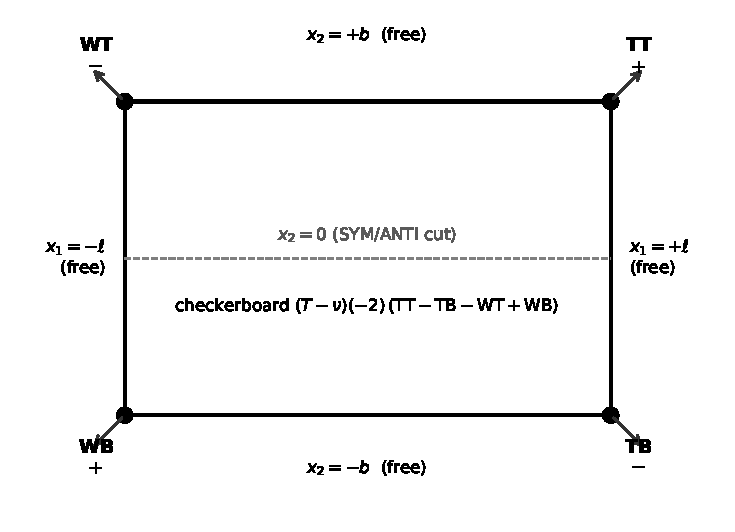
\includegraphics[width=0.78\linewidth]{rect_ffff_corner_checkerboard}
\caption{Completely free rectangle with outward normals at the four
corners. TT and WB enter the jump with a plus, TB and WT with a minus:
the checkerboard of Eq.~\eqref{eq:checkerboard}. The dashed line is the
half-model cut.}
\label{fig:checkerboard}
\end{figure}
A naive sum of four cantilever-style terms,
$p_{1t}q_{0t}+p_{1b}q_{0b}$ and cyclic, vanishes identically because those
two products sum to zero (parity identity). Under that identity the
checkerboard is twice the three-corner single-point combination that had
been used as an underived stand-in. The default cantilever assembly
(three free edges, one clamped) is a different contour and is not
altered.

The line-by-line contour trace, the four-corner table, the parity
identity in both classes, and the algebraic check that the checkerboard
is exactly twice the single-point candidate are Supplementary Material,
\S{}S.1.

\subsection{Screen B}\label{sec:screenb}
Discovery scans $\sigma_{\min}(\Lambda)$ on the production basis. Every
listed dip with $\sigma<0.3$ is re-scanned on the persist basis
($n_{\mathrm{cpair}}=3$, window $\pm 0.02$, step $0.002$). A dip
\textbf{persists} if a persist-basis local minimum remains within $0.01$
in $\Lambda$. That cut was frozen before the extra-$\ell/b$ geometries
were run and is not retuned. The same rule, with $\bar\Omega$ in place of
$\Lambda$ and the in-plane persist basis of \S\ref{sec:ipfe}, is applied
to the extensional candidates; what the rectangle has no analogue of is
the annular companion's \emph{residual} screen, not persistence itself.

Screen~B kills a recurring antisymmetric pair near $\Lambda=0.04$ and
$0.46$, and labels a symmetric leak at $0.41$ that persists but does not
match FE. It does not kill a deep extra near $\Lambda=1.65$ (tiny
$\sigma$, no FE partner) or a shallow symmetric extra near $1.92$. Those
are reported as false positives, not published modes.

Two genuine symmetric FE modes ($\ell/b=2.0$, $\Lambda=0.543$;
$\ell/b=3.0$, $\Lambda=0.670$) never appear as production-basis dips. On
the persist basis they sit on the FE values at $0.00\%$ miss. Production
discovery is therefore a floor, not a census: those two modes are
recovered by the persist screen, not by silently enlarging the published
detector.

A post-hoc sensitivity check replaces the fixed $0.002$-step persist
scan with a golden-section continuum minimisation at the same persist
basis. Two Table~\ref{tab:oop-high} entries -- $\ell/b=1.5$ SYM
$\Lambda^{*}=5.380$ and $\ell/b=2.5$ ANTI $\Lambda^{*}=6.260$ -- sit at
$|\Delta\Lambda|=0.0103$ and $0.0110$ at that continuum optimum, outside
the frozen $0.01$ cut by $3$--$10\%$, though within it under the
fixed-step scan that was actually run to discover them. The closest
extensional case ($\ell/b=3.0$ ANTI $\bar\Omega^{*}=2.2400$) stays inside
at $|\Delta\bar\Omega|=0.0094$. Screen~B's own margin is genuinely thin
for those two flexural entries; independent FE agreement is not
($0.03\%$ and $0.65\%$ miss respectively, Table~\ref{tab:oop-high}). The
cut is not retuned; the two entries are retained on the strength of that
independent FE match, and neither meets the shape bar of
\S\ref{sec:oop-mac}.

\section{Flexural finite-element comparison}\label{sec:oopfe}
Half-model SHELL281, $E=210\,\mathrm{GPa}$, $\nu=0.30$,
$\rho=7800\,\mathrm{kg\,m^{-3}}$, $H=0.04\,\mathrm{m}$, $b=1\,\mathrm{m}$.
Mesh~1 uses element size $b/20$ along the half-breadth; mesh~2 uses
$b/30$. Divisions along the length scale as
$\mathrm{NDIVX}=\mathrm{round}(2(\ell/b)\times 20)$ and $\times 30$.
Mesh~1 versus mesh~2 agrees to $<0.02\%$ on the older decks and
$0.001\%$ on $\ell/b=2.0$ and $3.0$. Rigid-body (near-zero Hz) entries
are discarded. Cross-parity matches are not counted. At $\ell/b=1.0$
(square plate) some SYM and ANTI FE frequencies coincide; that
degeneracy is physical.\footnote{Job-level detail: Supplementary
Material, \S{}S.4.}

A refined candidate is a \textbf{MATCH} if the production-basis local
minimum after a $\pm 0.04$, step-$0.002$ polish lies within $3\%$ of a
same-parity FE $\Lambda$, and Screen~B still passes. Double-dips that
share one FE partner count once (closer kept). High-$\Lambda$ discovery
uses a $5\%$ coarse cut, then drops machine zeros at $4.000$ and $6.000$
($\sigma\sim 10^{-18}$ to $10^{-22}$) and collapses doubles; the tables
below keep the $3\%$ subset unless noted.

\subsection{Primary refined matches
(\texorpdfstring{$\Lambda\lesssim 2.4$}{Lambda ~< 2.4})}\label{sec:oop-primary}
Table~\ref{tab:oop-primary} reports all $26$ primary refined flexural matches with $\Lambda\lesssim 2.4$ across the five aspect ratios.
\begin{table}[!htbp]\centering\scriptsize
\caption{Primary refined flexural matches ($\Lambda\lesssim 2.4$) against
half-model SHELL281. Persist-basis-only rows are marked; they never
appear as production-basis dips.}
\label{tab:oop-primary}
\setlength{\tabcolsep}{3pt}
\noindent\begin{minipage}[t]{0.49\textwidth}
\begin{tabularx}{\linewidth}{@{}rllrrX@{}}
\toprule
$\ell/b$ & class & $\Lambda^{*}$ & $\Lambda_{\mathrm{FE}}$ & miss & note \\
\midrule
1.0 & ANTI & 1.366 & 1.35288 & 0.97\% & \\
1.5 & SYM  & 0.964 & 0.96347 & 0.06\% & 1st SYM \\
1.5 & SYM  & 2.254 & 2.24373 & 0.46\% & \\
1.5 & ANTI & 0.906 & 0.89838 & 0.85\% & 1st ANTI \\
1.5 & ANTI & 2.124 & 2.07036 & 2.59\% & weakest primary \\
2.0 & SYM  & 0.5434 & 0.54338 & 0.00\% & persist basis only \\
2.0 & SYM  & 1.510 & 1.50735 & 0.18\% & \\
2.0 & SYM  & 2.234 & 2.22558 & 0.38\% & \\
2.0 & ANTI & 0.674 & 0.66858 & 0.81\% & 1st ANTI \\
2.0 & ANTI & 1.482 & 1.47069 & 0.77\% & \\
2.5 & SYM  & 0.348 & 0.34766 & 0.10\% & 1st SYM \\
2.5 & SYM  & 0.978 & 0.96559 & 1.29\% & \\
2.5 & SYM  & 1.888 & 1.88370 & 0.23\% & \\
\bottomrule
\end{tabularx}
\end{minipage}\hfill
\begin{minipage}[t]{0.49\textwidth}
\begin{tabularx}{\linewidth}{@{}rllrrX@{}}
\toprule
$\ell/b$ & class & $\Lambda^{*}$ & $\Lambda_{\mathrm{FE}}$ & miss & note \\
\midrule
2.5 & SYM  & 2.278 & 2.27059 & 0.33\% & \\
2.5 & ANTI & 0.534 & 0.53126 & 0.52\% & 1st ANTI \\
2.5 & ANTI & 1.148 & 1.14003 & 0.70\% & \\
2.5 & ANTI & 1.918 & 1.90392 & 0.74\% & \\
3.0 & SYM  & 0.242 & 0.24127 & 0.30\% & 1st SYM \\
3.0 & SYM  & 0.6698 & 0.66984 & 0.00\% & persist basis only \\
3.0 & SYM  & 1.320 & 1.31785 & 0.16\% & \\
3.0 & SYM  & 2.162 & 2.15417 & 0.36\% & \\
3.0 & SYM  & 2.256 & 2.24841 & 0.34\% & \\
3.0 & ANTI & 0.444 & 0.44044 & 0.81\% & 1st ANTI; $0.46$-family coincidence \\
3.0 & ANTI & 0.936 & 0.93044 & 0.60\% & \\
3.0 & ANTI & 1.528 & 1.51698 & 0.73\% & \\
3.0 & ANTI & 2.258 & 2.24305 & 0.67\% & \\
\bottomrule
\end{tabularx}
\end{minipage}
\end{table}
\FloatBarrier

First-mode travel, quoting Table~\ref{tab:oop-primary}'s $\Lambda^{*}$:
SYM $0.964\to 0.5434\to 0.348\to 0.242$ as $\ell/b$ goes
$1.5\to 2.0\to 2.5\to 3.0$ (the square plate's first SYM is the unmatched
$\Lambda_{\mathrm{FE}}=1.982$ of \S\ref{sec:oop-open}); ANTI
$1.366\to 0.906\to 0.674\to 0.534\to 0.444$ as $\ell/b$ goes
$1.0\to 1.5\to 2.0\to 2.5\to 3.0$. At $\ell/b=3.0$ the historical ANTI
$0.46$ leak sits on the real first ANTI; it is published as that mode
in Table~\ref{tab:oop-primary}, not as evidence that the leak is physical
at other aspect ratios.

\subsection{Higher flexural matches}\label{sec:oop-high}
Table~\ref{tab:oop-high} extends the comparison past that cutoff with $30$ further flexural matches at miss $\le 3\%$, giving $56$ published flexural rows in all.
\begin{table}[!htbp]\centering\footnotesize
\caption{Selected higher flexural matches with miss $\le 3\%$.
$^\ddagger$Persist-basis distance exceeds the frozen Screen~B cut at the
continuum optimum (\S\ref{sec:screenb}); retained on FE agreement.
Neither row meets the shape bar of \S\ref{sec:oop-mac}.}
\label{tab:oop-high}
\setlength{\tabcolsep}{5pt}
\noindent\begin{minipage}[t]{0.49\textwidth}
\begin{tabular}{@{}rllrr@{}}
\toprule
$\ell/b$ & class & $\Lambda^{*}$ & $\Lambda_{\mathrm{FE}}$ & miss \\
\midrule
1.0 & SYM  & 2.460 & 2.45439 & 0.23\% \\
1.0 & SYM  & 3.530 & 3.49250 & 1.07\% \\
1.0 & SYM  & 6.190 & 6.16026 & 0.48\% \\
1.0 & SYM  & 6.460 & 6.36553 & 1.48\% \\
1.0 & ANTI & 3.520 & 3.49250 & 0.79\% \\
1.5 & SYM  & 5.380$^\ddagger$ & 5.38152 & 0.03\% \\
1.5 & ANTI & 3.860 & 3.83354 & 0.69\% \\
2.0 & SYM  & 3.000 & 2.99812 & 0.06\% \\
2.0 & SYM  & 3.650 & 3.62227 & 0.77\% \\
2.0 & ANTI & 2.580 & 2.55180 & 1.11\% \\
2.0 & ANTI & 4.060 & 4.02613 & 0.84\% \\
2.0 & ANTI & 6.200 & 6.17866 & 0.35\% \\
2.5 & SYM  & 3.190 & 3.19522 & 0.16\% \\
2.5 & SYM  & 4.180 & 4.13819 & 1.01\% \\
2.5 & SYM  & 5.410 & 5.34819 & 1.16\% \\
\bottomrule
\end{tabular}
\end{minipage}\hfill
\begin{minipage}[t]{0.49\textwidth}
\begin{tabular}{@{}rllrr@{}}
\toprule
$\ell/b$ & class & $\Lambda^{*}$ & $\Lambda_{\mathrm{FE}}$ & miss \\
\midrule
2.5 & ANTI & 2.920 & 2.89206 & 0.97\% \\
2.5 & ANTI & 4.180 & 4.14962 & 0.73\% \\
2.5 & ANTI & 5.720 & 5.67275 & 0.83\% \\
2.5 & ANTI & 6.260$^\ddagger$ & 6.21965 & 0.65\% \\
2.5 & ANTI & 6.400 & 6.36131 & 0.61\% \\
3.0 & SYM  & 2.480 & 2.45935 & 0.84\% \\
3.0 & SYM  & 3.340 & 3.32528 & 0.44\% \\
3.0 & SYM  & 3.660 & 3.62467 & 0.97\% \\
3.0 & SYM  & 5.660 & 5.59746 & 1.12\% \\
3.0 & SYM  & 6.180 & 6.14744 & 0.53\% \\
3.0 & ANTI & 3.160 & 3.14253 & 0.56\% \\
3.0 & ANTI & 4.260 & 4.23529 & 0.58\% \\
3.0 & ANTI & 5.560 & 5.51872 & 0.75\% \\
3.0 & ANTI & 6.220 & 6.18191 & 0.62\% \\
3.0 & ANTI & 6.380 & 6.34339 & 0.58\% \\
\bottomrule
\end{tabular}
\end{minipage}
\end{table}
\FloatBarrier

\subsection{Eigenvector cross-check (MAC)}\label{sec:oop-mac}
Frequency agreement does not by itself identify a mode. For each
published $\Lambda^{*}$ the analytical $w$ is reconstructed from the
null vector of the free-free characteristic matrix and scored against
the same-parity half-model SHELL281 $U_Z$ eigenvector at the matching
$\Lambda_{\mathrm{FE}}$, using the identity-weighted MAC
$|\langle u_Z,w\rangle|^2/(\|u_Z\|^2\|w\|^2)$ of Allemang
\cite{allemang2003}, the same form used in the annular companion
\cite{mccune2026annular}. The bar $0.744$ is that paper's production
call (the midpoint of its $\nu=0.30$ extensional calibration window),
applied here unre-tuned as a conservative shape-confirmation threshold,
not as a new calibration against these data. FE
hertz are converted in Python with $K=24.6644$; the decks' own printed
$\Lambda$ column is not used.

Of the $56$ published flexural rows of
Tables~\ref{tab:oop-primary}--\ref{tab:oop-high}, $36$ meet the bar:
$25$ of $29$ symmetric and $11$ of $27$ antisymmetric. The other $20$ are
frequency matches only and no shape is claimed for them.

Isolated primary matches confirm: every first symmetric mode has
MAC${}\ge 0.959$, and four of the five first antisymmetric modes lie at
or above the bar (the $\ell/b=2.5$ first ANTI saturates at $0.655$
across a fine $\Lambda$ grid, so the frequency match stands and the
shape is reported as ambiguous). The bar's placement is not delicate: no
row lies between $0.655$, the highest MAC reached by an excluded row, and
$0.751$, the lowest confirmed one, so the confirmed set is the same for
any threshold in that interval.
Known Screen~B leaks split: the SYM $0.41$ family has
MAC${}\le 0.05$ against every same-parity FE mode; the ANTI $0.46$
family stays below the $0.744$ bar (MAC $0.19$--$0.43$) except at
$\ell/b=3.0$, where it coincides with the real first ANTI and scores
$1.000$ as that mode. At
$\ell/b=2.5$ a $1\%$ FE pair ($3.16376$ and $3.19522$) is
frequency-nearest-matched to $\Lambda^{*}=3.190\to 3.19522$; the
production-basis shape attaches to $3.16376$, and an
$n_{\mathrm{cpair}}=6$ reconstruction returns MAC $=0.915$ against
$3.19522$, so the published frequency partner is the one the enlarged
basis selects. Higher-$\Lambda$ reconstructions can land on a nearby
kernel or on the known machine-zero at $\Lambda=4,6$; those frequency
matches are not withdrawn. The confirmed rows and the reconstruction
basis used for each are Supplementary Material, \S{}S.5.\footnote{Job-level
detail: Supplementary Material, \S{}S.4.}
Figure~\ref{fig:mac-overlay} is the first symmetric mode at
$\ell/b=1.5$: production-basis $w$ against the matching SHELL281 $U_Z$,
MAC $=1.000$. A dps$=40$ persist-basis golden-section polish of the
seven Table~\ref{tab:oop-primary} ANTI rows that do not meet the bar
converges to the published $\Lambda^{*}$ (max travel $8\times 10^{-4}$)
and does not lift persist-basis MAC across $0.744$, so coarseness of
$\Lambda^{*}$ is not what holds those rows below it, and the bar is not
retuned.

\begin{figure}[!htbp]\centering
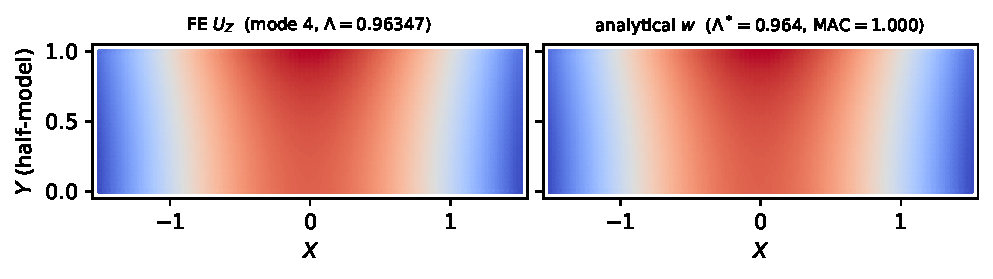
\includegraphics[width=\linewidth]{rect_ff_oop_mac_lb15_sym0964}
\caption{Half-model first symmetric flexural mode at $\ell/b=1.5$.
Left: SHELL281 $U_Z$ (mode 4, $\Lambda_{\mathrm{FE}}=0.96347$).
Right: analytical $w$ at $\Lambda^{*}=0.964$, MAC $=1.000$.}
\label{fig:mac-overlay}
\end{figure}

\subsection{Open flexural items}\label{sec:oop-open}
\begin{itemize}\itemsep2pt
\item $\ell/b=1.0$ SYM $\Lambda_{\mathrm{FE}}=1.982$: unmatched, closed as
a numerical curiosity. A persist-basis scan over $[1.73,2.23]$ stays
within one order of magnitude of its floor (ratio $3.12$), with no dip
near $1.982$ and no tail toward the next SYM root at $2.454$ (matched
separately by $\Lambda=2.460$). Not a missing mode; Screen~B is not
retuned.
\item $\ell/b=1.5$ ANTI $\Lambda^{*}=2.124$ (Leissa $(3,2)$, miss
$2.59\%$) is the weakest primary frequency match and does not MAC-
confirm against FE\#5 even at $n_{\mathrm{cpair}}=6$. The frequency
row is kept; the shape is not claimed.
\item Several FE modes near $2.5$--$2.9$ fail Screen~B even when a
production dip is within ${\sim}1.5\%$ (e.g.\ $2.0$ SYM $2.622$, $3.0$
SYM $2.887$, $1.5$ SYM $2.588$, $2.5$ SYM $2.467$). The screen is not
retuned to collect them.
\item Not published: SYM $0.41$ leak; ANTI $0.04/0.46$ except the
$\ell/b=3.0$ coincidence above; ANTI ${\sim}1.65$; shallow SYM
${\sim}1.92$; $\Lambda=4,6$ machine zeros.
\end{itemize}

\subsection{Comparison with Leissa (1973)}\label{sec:leissa}
Leissa's Rayleigh--Ritz survey of rectangular-plate vibration \cite{leissa1973}
tabulates F--F--F--F frequency parameters $\lambda=\omega a^2\sqrt{\rho h/D}$
(Table C15 of that reference) at five aspect ratios, three of which,
$a/b=1.0,1.5,2.5$, coincide with the flexural aspect ratios used here. Using
$a=2\ell$, $D=Eh^3/[12(1-\nu^2)]$ and the same $H=0.04\,$m, $E=210\,$GPa,
$\rho=7800\,\mathrm{kg\,m^{-3}}$ as \S\ref{sec:oopfe}, $\lambda$ converts to
$\Lambda$ through $\Lambda = (\lambda/a^2)/(2\pi K\sqrt{\rho h/D})$, using the
same $K=24.6644\,$Hz-per-unit-$\Lambda$ constant as the finite-element
comparison. The conversion is self-consistent to $0.05\%$ on the one entry
independently checkable against the published $\Lambda^{*}=1.366$
($\ell/b=1.0$, ANTI): Leissa's fundamental $(2,2)$ mode,
$\lambda=13.489$, converts to $\Lambda=1.3667$.

Leissa's own $(m,n)$ half-wave counts fix the parity: odd $n$ is
$y$-symmetric, which is SYM here, and even $n$ is $y$-antisymmetric, which
is ANTI. Table~\ref{tab:leissa} reports every Leissa entry in those three
columns that converts within $2\%$ of a \emph{same-parity}
$\Lambda_{\mathrm{FE}}$ already listed in
Tables~\ref{tab:oop-primary}--\ref{tab:oop-high}; pairing is by parity,
not by nearest frequency.

\begin{table}[!htbp]
\centering\footnotesize
\caption{Flexural matches against Leissa (1973), Table C15, converted as
above and paired by parity. The $(m,n)$ column is Leissa's own half-wave
count (odd $n$: $y$-symmetric $=$ SYM here; even $n$: $y$-antisymmetric $=$
ANTI). Miss is
$|\Lambda^{*}-\Lambda_{\text{Leissa}}|/\Lambda_{\text{Leissa}}$, the same
convention as Table~\ref{tab:bardell}.}\label{tab:leissa}
\setlength{\tabcolsep}{4pt}
\begin{tabular}{@{}rllrrrr@{}}
\toprule
$\ell/b$ & class & $(m,n)$ & $\Lambda_{\text{Leissa}}$ & $\Lambda^{*}$ & $\Lambda_{\mathrm{FE}}$ & miss \\
\midrule
1.0 & ANTI & $(2,2)$ & 1.3667 & 1.366 & 1.35288 & 0.05\% \\
1.0 & SYM  & $(3,1)$ & 2.4755 & 2.460 & 2.45439 & 0.63\% \\
1.0 & ANTI & $(3,2)$ & 3.5487 & 3.520 & 3.49250 & 0.81\% \\
1.0 & SYM  & $(2,3)$ & 3.5487 & 3.530 & 3.49250 & 0.53\% \\
1.0 & SYM  & $(4,1)$ & 6.2339 & 6.190 & 6.16026 & 0.70\% \\
1.5 & ANTI & $(2,2)$ & 0.9064 & 0.906 & 0.89838 & 0.04\% \\
1.5 & SYM  & $(3,1)$ & 0.9728 & 0.964 & 0.96347 & 0.91\% \\
1.5 & ANTI & $(3,2)$ & 2.1009 & 2.124 & 2.07036 & 1.10\% \\
1.5 & SYM  & $(1,3)$ & 2.2648 & 2.254 & 2.24373 & 0.48\% \\
2.5 & SYM  & $(3,1)$ & 0.3509 & 0.348 & 0.34766 & 0.82\% \\
2.5 & ANTI & $(2,2)$ & 0.5358 & 0.534 & 0.53126 & 0.33\% \\
2.5 & SYM  & $(4,1)$ & 0.9749 & 0.978 & 0.96559 & 0.32\% \\
2.5 & ANTI & $(3,2)$ & 1.1589 & 1.148 & 1.14003 & 0.94\% \\
2.5 & SYM  & $(5,1)$ & 1.9040 & 1.888 & 1.88370 & 0.84\% \\
2.5 & ANTI & $(4,2)$ & 1.9353 & 1.918 & 1.90392 & 0.89\% \\
\bottomrule
\end{tabular}
\end{table}

All fifteen conversions land within $1.10\%$ of the matched root
$\Lambda^{*}$, using no information from this paper's own solver beyond the
conversion constant $K$; the independent finite-element values agree with
the same fifteen entries to within $1.62\%$. The two eigenvalues Leissa
lists at $\lambda=35.024$ for the square plate reproduce the SYM/ANTI
degeneracy this paper's own FE and solver both find there, and enter as the
$(3,2)$ and $(2,3)$ rows.

Parity, rather than frequency, does real work at $\ell/b=2.5$, where
Leissa's $(5,1)$ ($\lambda=117.45$, $y$-symmetric) converts to
$\Lambda=1.9040$ and his $(4,2)$ ($\lambda=119.38$, $y$-antisymmetric) to
$1.9353$, while this paper's SYM and ANTI FE values sit at $1.88370$ and
$1.90392$. Nearest-frequency matching would pair the $y$-symmetric
$(5,1)$ with the antisymmetric FE mode at $0.005\%$ and leave $(4,2)$
unaccounted for. Table~\ref{tab:leissa} pairs each with its own parity
instead: the agreement is $0.84\%$ and $0.89\%$ rather than $0.005\%$, and
every row in the table is a same-parity comparison.

Three further Leissa entries in these three columns convert close to a
finite-element mode that Tables~\ref{tab:oop-primary}--\ref{tab:oop-high}
do not contain. Leissa's second $\ell/b=1.0$ mode ($\lambda=19.789$, whose
quoted internal convergence check at $13.06\%$ is the worst-behaved of that
column) converts to $\Lambda=2.0050$, $1.12\%$ from the $\ell/b=1.0$ SYM
$\Lambda_{\mathrm{FE}}=1.98249$ named in \S\ref{sec:oop-open} as an
unmatched curiosity: an independent Ritz solution also struggles with this
mode, which weighs against it being an artifact of this paper's own
screening. Leissa's $\ell/b=1.5$ $\lambda=58.201$ converts to
$\Lambda=2.6209$, $1.25\%$ from the FE mode at $2.58809$ named in
\S\ref{sec:oop-open} as failing Screen~B despite a nearby production dip,
so the literature value corroborates that a real mode sits there. His
$\ell/b=1.5$ $\lambda=67.494$ converts to $\Lambda=3.0394$, $1.17\%$ from
the FE mode at $3.00395$, which likewise has no published match.

\section{In-plane motion}\label{sec:ip}

\subsection{No Kirchhoff corner jump}\label{sec:ip-corner}
Seok, Tiersten and Scarton Part~2 Eq.~(1) is Part~1 Eq.~(16) with flexure
set to zero: only $\int_{c_N} n_a t^{(0)}_{ab}\delta u_b\,ds$ and
$\int_{c_C} u_b\delta(n_a t^{(0)}_{ab})\,ds$ remain on the boundary. The
twisting-moment exact differential that produces the out-of-plane corner
jump is absent. After the long free edges are satisfied exactly, Eq.~(36)
is wall (clamped) plus tip (free traction) only. The in-plane assembler
is that form ($\mathbf{K}=\mathrm{wall}+\mathrm{tip}$); the class has no
corner term. Completely free in-plane motion is the same two traction
integrals on both short edges --- still no jump. The free-free option is
an edge-list swap, not a new formula. Default clamped-free assembly is
bit-identical to the cantilever path.

\subsection{Finite-element comparison}\label{sec:ipfe}
Half-model PLANE183, same geometry and material as \S\ref{sec:oopfe}, at
$\ell/b=1.0,1.5,2.0,2.5,3.0$. Mesh~1 versus mesh~2 agrees to $0.004\%$.
Rigid-body (near-zero Hz) entries are discarded. The
Seok/Tiersten/Scarton in-plane parameter is
$\bar\Omega=\omega/\bar\omega$,
$\bar\omega=(\pi/(2b))\sqrt{c_{66}/\rho}$,
$c_{66}=E/[2(1+\nu)]$. Finite-element comparisons convert ANSYS cyclic
frequencies by $\bar\Omega=f/804.481\,\mathrm{Hz}$, independent of
$\ell/b$. SYM $\leftrightarrow$ $UY=0$ on the cut; ANTI
$\leftrightarrow$ $UX=0$. Conversion constants and the full 92-row match
list are Supplementary Material, \S\S{}S.2--S.3.

Production in-plane discovery uses the persist-sized basis
($n_{\mathrm{real}}=5$, $n_{\mathrm{cpair}}=3$) directly, not the
cantilever default $n_{\mathrm{cpair}}=0$: that default starves the FFFF
spectrum (a band of real FE targets produced no dip at all until the
basis was enlarged). A candidate is a \textbf{MATCH} if a same-basis
local minimum after a $\pm 0.02$, step-$0.002$ polish lies within $3\%$
of a same-parity FE $\bar\Omega$. Sixteen FE targets that the
$n_{\mathrm{cpair}}=3$ scan left uncovered recover at
$n_{\mathrm{cpair}}=5$ in a $\pm 0.05$ window centred on the FE value
itself (15 at $0.00\%$ miss, one at $0.14\%$). This is \textbf{not}
Screen~B and is not adopted as a portable residual screen. The annular
companion's SUBDOM instrument \cite{mccune2026annular} remains
annular-IP-specific.

After collapsing double-dips onto the same FE partner, \textbf{every} one
of the 92 unique non-rigid FE targets in $\bar\Omega\in[0.02,2.50]$
($5+4+8+6+10+7+13+10+16+13$ across the five aspect ratios and both
parities) has a matched root; zero remain uncovered. Sixteen of the 92 are
the enlarged-basis recoveries above, found in a window centred on the
finite-element value rather than by blind discovery, and are tagged as such
in the full list. First-mode travel of the
matched $\bar\Omega^{*}$ is regular: SYM
$1.330\to 1.050\to 0.810\to 0.640\to 0.540$ and ANTI
$1.240\to 0.780\to 0.520\to 0.380\to 0.280$ as $\ell/b$ goes
$1.0\to 1.5\to 2.0\to 2.5\to 3.0$.

\textbf{No eigenvector cross-check is presented for the in-plane family.}
The resolved branch pool near several in-plane frequencies is thin --- three
to five candidates --- and largely insensitive to the width of the branch
search, so a reconstruction there would not carry the confirm/reject
separation that makes the flexural comparison of \S\ref{sec:oop-mac}
informative. The in-plane result in this paper is a frequency census
against independent finite elements and against
\S\ref{sec:bardell}--\S\ref{sec:gorman}; nothing is claimed about
in-plane mode shapes.

\subsection{Comparison with Bardell, Langley and Dunsdon (1996)}\label{sec:bardell}
Bardell, Langley and Dunsdon \cite{bardell1996} give the first six
non-zero in-plane frequencies of isotropic F--F--F--F rectangles at
$a/b=1$ and $2$, printed under Figure~1 mode plots rather than tabulated
(their one table is a simply-supported convergence study). Their
parameter is $\Omega_B=\omega a/C_L$ with $C_L^2=E/[\rho(1-\nu^2)]$. The
letter does not state $\nu$ numerically; their own Table~1, an exact
S--S--S--S convergence study, gives the square-plate pair
$(0,1)=(1,0)=1.859$, which equals $\pi\sqrt{(1-\nu)/2}=1.8586$ at
$\nu=0.30$, so the conversion uses that value.

The plates identify as $a=2\ell$, so $a/b=\ell/b$ and
\begin{equation}
\Omega_B=\bar\Omega\cdot\pi\cdot(\ell/b)\cdot\sqrt{(1-\nu)/2}.
\label{eq:bardell-conv}
\end{equation}
Figure~1's caption reads ``(a)~$a/b=1$; (b)~$a/b=2$'', but the (a)
panel is drawn 2:1 with unique frequencies and the (b) panel is square
with the repeated pair $2.472,2.472$. The body text assigns repeats to
$a/b=1$ and unique frequencies to $a/b=2$. The mapping below follows the
rendered proportions and that physics, not the caption letters (the
annular companion \cite{mccune2026annular} recorded the same defect; the
source's own Table~1 does not have it). Supplementary Material \S{}S.2
restates the mapping.

\begin{table}[!htbp]\centering\footnotesize
\caption{Bardell, Langley and Dunsdon \cite{bardell1996} F--F--F--F first
six non-zero frequencies at $a/b=1$ and $2$, converted onto this paper's
$\bar\Omega$ and paired with the matched root and independent FE.
Miss is $|\bar\Omega^{*}-\Omega_B^{\mathrm{conv}}|/\Omega_B^{\mathrm{conv}}$.
Aspect ratios are assigned by plate proportions (square $+$ repeated
$2.472$ $=a/b=1$), not Figure~1's (a)/(b) caption letters.}
\label{tab:bardell}
\setlength{\tabcolsep}{4pt}
\begin{tabular}{@{}rlrrrrr@{}}
\toprule
$\ell/b$ & class & Bardell $\Omega_B$ & $\Omega_B\to\bar\Omega$ & $\bar\Omega^{*}$ & $\bar\Omega_{\mathrm{FE}}$ & miss \\
\midrule
1.0 & ANTI & 2.321 & 1.24880 & 1.2400 & 1.24858 & 0.70\% \\
1.0 & SYM  & 2.472 & 1.33004 & 1.3300 & 1.32984 & 0.00\% \\
1.0 & ANTI & 2.472 & 1.33004 & 1.3298 & 1.32984 & 0.02\% \\
1.0 & SYM  & 2.628 & 1.41397 & 1.4100 & 1.41422 & 0.28\% \\
1.0 & SYM  & 2.987 & 1.60713 & 1.6100 & 1.60733 & 0.18\% \\
1.0 & SYM  & 3.452 & 1.85732 & 1.8600 & 1.85745 & 0.14\% \\
2.0 & ANTI & 1.954 & 0.52567 & 0.5200 & 0.52557 & 1.08\% \\
2.0 & SYM  & 2.961 & 0.79657 & 0.8100 & 0.79652 & 1.69\% \\
2.0 & ANTI & 3.267 & 0.87889 & 0.8800 & 0.87891 & 0.13\% \\
2.0 & ANTI & 4.726 & 1.27139 & 1.2715 & 1.27148 & 0.01\% \\
2.0 & ANTI & 4.784 & 1.28700 & 1.2800 & 1.28703 & 0.54\% \\
2.0 & SYM  & 5.205 & 1.40025 & 1.4000 & 1.40011 & 0.02\% \\
\bottomrule
\end{tabular}
\end{table}

All twelve published F--F--F--F values are matched. Solver versus
converted Bardell: max miss $1.69\%$, eight of twelve inside $0.3\%$.
Independent FE versus converted Bardell: max miss $0.019\%$. The three
largest solver misses sit on $n_{\mathrm{cpair}}=3$ roots that already
passed the $3\%$ FE cut on the refine grid (printed $\bar\Omega^{*}$ to
$0.01$); the two $n_{\mathrm{cpair}}=5$ mop-up roots that fall inside
Bardell's first six sit at $0.01$--$0.02\%$. The repeated square-plate
pair $2.472,2.472$ is the SYM/ANTI degeneracy at
$\bar\Omega_{\mathrm{FE}}=1.32984$.

\subsection{Comparison with Gorman (2004)}\label{sec:gorman}
Gorman's superposition-method solution for in-plane vibration of the
completely free rectangular plate \cite{gorman2004} tabulates
symmetric--symmetric, antisymmetric--antisymmetric, and mixed-parity mode
families separately at the square plate and at one rectangular aspect
ratio, $b/a=0.5$, i.e. $a/b=2$, coinciding with $\ell/b=1.0$ and $\ell/b=2.0$
here. Gorman's own tables already cross-check against Bardell's values
directly (his ``Ref.~[1]''); comparing them against the present solver
independently triangulates three separate methods.

One conversion subtlety was found and is recorded here for reproducibility.
Gorman's tabulated $\lambda^2$ column is numerically \emph{half} of the
equivalent Bardell $\bar\Omega_B$ for the same mode (e.g. Gorman's
$\lambda^2=1.160$ for the square plate's first symmetric--symmetric mode
converts, after doubling, to $\Omega_B=2.320$, matching Bardell's own
published $2.321$ for that mode to four figures) despite both papers
quoting an apparently identical formula $\lambda^2=\omega a\sqrt{\rho(1-\nu^2)/E}$:
Gorman's quarter-plate schematic (his Fig.~2) evidently uses $a$ as the
\emph{half}-length rather than the full edge length assumed by the
nomenclature list. Doubling Gorman's tabulated values before applying
Eq.~\eqref{eq:bardell-conv} resolves the discrepancy to within FE-level agreement (below);
using Gorman's values unconverted would have understated every frequency
by very nearly a factor of two.

\begin{table}[!htbp]
\centering\footnotesize
\caption{In-plane matches against Gorman (2004), doubled and converted via
Eq.~\eqref{eq:bardell-conv}. Miss is
$|\bar\Omega^{*}-\bar\Omega_{\text{Gorman}}|/\bar\Omega_{\text{Gorman}}$,
the same convention as Table~\ref{tab:bardell}; it is computed before
$\bar\Omega_{\text{Gorman}}$ is rounded to the four places shown. The class
column is this paper's half-model parity, which is the opposite label to
Gorman's quarter-plate family names (his symmetric--symmetric modes are ANTI
here); pairing follows the finite-element parity, not his
nomenclature.}\label{tab:gorman}
\setlength{\tabcolsep}{4pt}
\begin{tabular}{@{}rlrrrr@{}}
\toprule
$\ell/b$ & class & $\bar\Omega_{\text{Gorman}}$ & $\bar\Omega^{*}$ & $\bar\Omega_{\mathrm{FE}}$ & miss \\
\midrule
1.0 & ANTI & 1.2483 & 1.2400 & 1.24858 & 0.66\% \\
1.0 & SYM/ANTI (degenerate) & 1.3300 & 1.3300/1.3298 & 1.32984 & 0.02\% \\
1.0 & SYM  & 1.4140 & 1.4100 & 1.41422 & 0.28\% \\
1.0 & SYM  & 1.6077 & 1.6100 & 1.60733 & 0.14\% \\
1.0 & SYM  & 1.8573 & 1.8600 & 1.85745 & 0.14\% \\
1.0 & SYM/ANTI (degenerate) & 2.0037 & 2.0000 & 2.00319 & 0.18\% \\
1.0 & ANTI & 2.3168 & 2.3200 & 2.31523 & 0.14\% \\
2.0 & ANTI & 0.5262 & 0.5200 & 0.52557 & 1.17\% \\
2.0 & SYM  & 0.7963 & 0.8100 & 0.79652 & 1.72\% \\
2.0 & ANTI & 0.8792 & 0.8800 & 0.87891 & 0.10\% \\
2.0 & ANTI & 1.2714 & 1.2715 & 1.27148 & 0.01\% \\
2.0 & ANTI & 1.2870 & 1.2800 & 1.28703 & 0.54\% \\
2.0 & SYM  & 1.4011 & 1.4000 & 1.40011 & 0.08\% \\
2.0 & SYM  & 1.4145 & 1.4142 & 1.41422 & 0.02\% \\
2.0 & SYM  & 1.4446 & 1.4400 & 1.44333 & 0.32\% \\
2.0 & SYM  & 1.6539 & 1.6500 & 1.65355 & 0.24\% \\
2.0 & SYM  & 1.7745 & 1.7500 & 1.77390 & 1.38\% \\
2.0 & ANTI & 1.8444 & 1.8400 & 1.84467 & 0.24\% \\
2.0 & ANTI & 2.1382 & 2.1400 & 2.13652 & 0.09\% \\
\bottomrule
\end{tabular}
\end{table}

Nineteen of Gorman's twenty-four tabulated eigenvalues land inside the
$\bar\Omega\in[0.02,2.50]$ window covered by the full in-plane match list
(Supplementary \S{}S.3). All nineteen match a published root within
$1.72\%$, and the independent finite-element values agree with the same
nineteen to within $0.11\%$. The two largest solver misses, $1.72\%$ and
$1.38\%$ at $\ell/b=2.0$, are the same $n_{\mathrm{cpair}}=3$ discovery
roots printed to $0.01$ that carry the largest Bardell misses; the FE
column shows the underlying agreement is far tighter than the printed
resolution of $\bar\Omega^{*}$. That the finite-element values reproduce
Bardell to $0.019\%$ and Gorman to $0.11\%$ is consistent with the two
being, by Gorman's own account, independent confirmations of each other.
The remaining five Gorman eigenvalues, all at $\ell/b=1.0$ (Gorman
tabulates only four modes per family there, and the higher-parity ones run
past $\bar\Omega=2.5$), exceed the FE window's upper cutoff and are not
compared.

\section{Discussion}\label{sec:disc}
The four-corner jump is a derivation rather than a fit; Screen~B is
frozen; five aspect ratios of independent FE agree at the level the
annular flexural tables claimed \cite{mccune2026annular}. The remaining
flexural issues are named misses and named artifacts.

The two papers split instruments as well as geometry. The annular
companion screens a two-edge Galerkin projection by pointwise residuals
(two-sided in flexure; one-sided in extension, closed by SUBDOM and by
the MAC bar reused here). After the long edges of the rectangle are
satisfied exactly, that residual taxonomy has nothing to act on: the
remaining defect is a mixture of basis-limited dips and a few
$\ell/b$-independent leak families, which is why \S\ref{sec:screenb}
uses persistence instead of a residual cut. What the rectangle has no
analogue of is the residual screen itself, in either motion family: the
persistence rule of \S\ref{sec:screenb} is applied to the flexural and
extensional candidates alike, while SUBDOM stays annular-IP-specific.
Completely free in-plane motion on the rectangle also has no Kirchhoff
jump, and what its result rests on is the 92/92 frequency census together
with Bardell and Gorman --- a frequency claim, with no shape cross-check
behind it.

What this paper does \emph{not} claim: that production-basis flexural
discovery is complete; that the in-plane matches are shape-confirmed; that
the unre-tuned MAC bar is a new calibration on these data.

This paper is the rectangular companion of the annular manuscript, not
an expansion of it. The annular contribution is the two-edge FFFF
detector and its discrimination instruments on a sector. This paper's
contribution is the four-free-edge rectangular jump, the in-plane
edge-list extension that needs no jump, and the tables that follow from
both.

\section{Conclusions}\label{sec:conc}
The Seok--Tiersten--Scarton rectangular method extends to completely free
flexure once the closed-contour Kirchhoff jump is assembled as a
checkerboard rather than a vanishing four-term sum. A frozen complex-pair
persistence screen, checked against half-model SHELL281 at
$\ell/b=1.0,1.5,2.0,2.5,3.0$, yields a set of even- and odd-parity
frequencies that match FE typically inside $1\%$. Two symmetric modes
require the persist basis to appear; one square-plate symmetric target is
a named unmatched curiosity, not a missing mode. The same assembler
extends to completely free in-plane motion with no corner term.
Half-model PLANE183 at the five flexural aspect ratios matches every
non-rigid target in $\bar\Omega\in[0.02,2.50]$: 92 unique frequencies,
sixteen of them recovered at an enlarged basis in a window centred on the
finite-element value rather than by blind discovery.

Three independent literature sets bracket those tables. Bardell, Langley
and Dunsdon's 1996 first six F--F--F--F frequencies at $a/b=1,2$, converted
onto $\bar\Omega$, agree with the matched roots to at most $1.69\%$;
fifteen entries of Leissa's F--F--F--F table agree with the flexural roots
to at most $1.10\%$; nineteen of Gorman's superposition eigenvalues agree
to at most $1.72\%$. Measured instead against the independent
finite-element values, those same three sets agree to $0.019\%$, $1.62\%$
and $0.11\%$.

Shape validation is flexural only. MAC against the half-model $U_Z$
eigenvectors confirms 36 of the 56 published flexural rows, every first
symmetric mode among them at MAC${}\ge 0.959$, and the known Screen~B
leaks stay below the bar except where a leak frequency coincides with a
physical mode. No in-plane eigenvector comparison is presented. The elastic
FFFF baseline on both the annular \cite{mccune2026annular} and rectangular
geometries is the intended foundation for piezoelectric constitutive
coupling and for using the exact frequencies to identify those constants;
that is later work, not a claim of this paper.

\small
\section*{Data and code availability}
The solver, finite-element decks, validated tables, and from-scratch
regression suite are released under an MIT license as a public GitHub
repository, \url{https://github.com/McCune1/plate_solver}. For the present
paper that includes the free-free assembler, the Screen~B implementation
and every production probe behind
Tables~\ref{tab:oop-primary}--\ref{tab:gorman}, the APDL decks and their
frequency listings at all five aspect ratios, and regression gates for both
free-free rectangular assemblers; the per-mode nodal eigenvector dumps
behind \S\ref{sec:oop-mac} are roughly $88$\,MB and are regenerable from
the shipped mode-extraction decks rather than tracked. The public
tag \texttt{v1.0.0} matches the annular companion manuscript
\cite{mccune2026annular}; a manuscript-matching tag for the present
rectangular paper will be added at submission. Tables here were captured under
\texttt{SOLVER\_VERSION} \texttt{2026-07-10.s10}. Results under a
different version should be checked against the clamped-free regression
gates first. The four-corner derivation is Supplementary Material, \S{}S.1;
in-plane conversion constants and the 92-row match list are \S\S{}S.2--S.3;
cluster job numbers are \S{}S.4; the flexural MAC table is \S{}S.5.

\section*{Declaration of competing interests}
The authors declare that they have no known competing financial interests
or personal relationships that could have appeared to influence the work
reported in this paper.

\section*{Funding}
This research did not receive any specific grant from funding agencies in
the public, commercial, or not-for-profit sectors.

\section*{Acknowledgments}
The computation for this work was performed on The Mill HPC cluster at
Missouri University of Science and Technology \cite{mill2024}, using up
to 32 CPU cores per job. GPU resources were not used.

\section*{CRediT authorship contribution statement}
\textbf{Garrek McCune:} Conceptualization, Methodology, Software,
Validation, Formal analysis, Investigation, Writing -- original draft,
Writing -- review \& editing, Visualization. \textbf{Daniel Stutts:}
Conceptualization, Supervision.

\section*{Declaration of generative AI and AI-assisted technologies}
During the preparation of this work, the authors used generative AI tools
to assist with manuscript and code organization, drafting, editing, and
formatting. After using these tools, the authors reviewed and edited the
content as needed and take full responsibility for the content of this
publication.
\normalsize

\begin{thebibliography}{99}\small
\setlength{\itemsep}{0pt}
\setlength{\parsep}{0pt}
\bibitem{seok1} J. Seok, H.F. Tiersten, ``Free vibrations of annular sector
cantilever plates. Part 1: out-of-plane motion,'' J. Sound Vib. 271 (2004)
757--772. \url{https://doi.org/10.1016/S0022-460X(03)00414-0}.
\bibitem{seok2} J. Seok, H.F. Tiersten, ``Free vibrations of annular sector
cantilever plates. Part 2: in-plane motion,'' J. Sound Vib. 271 (2004)
773--787. \url{https://doi.org/10.1016/S0022-460X(03)00415-2}.
\bibitem{seok3} J. Seok, H.F. Tiersten, H.A. Scarton, ``Free vibrations of
rectangular cantilever plates. Part 1: out-of-plane motion,'' J. Sound
Vib. 271 (2004) 131--146. \url{https://doi.org/10.1016/S0022-460X(03)00365-1}.
\bibitem{seok4} J. Seok, H.F. Tiersten, H.A. Scarton, ``Free vibrations of
rectangular cantilever plates. Part 2: in-plane motion,'' J. Sound Vib.
271 (2004) 147--158. \url{https://doi.org/10.1016/S0022-460X(03)00366-3}.
\bibitem{bardell1996} N.S. Bardell, R.S. Langley, J.M. Dunsdon, ``On the
free in-plane vibration of isotropic rectangular plates,'' J. Sound Vib.
191 (3) (1996) 459--467. \url{https://doi.org/10.1006/jsvi.1996.0134}.
\bibitem{leissa1973} A.W. Leissa, ``The free vibration of rectangular
plates,'' J. Sound Vib. 31 (3) (1973) 257--293.
\url{https://doi.org/10.1016/S0022-460X(73)80371-2}.
\bibitem{gorman2004} D.J. Gorman, ``Free in-plane vibration analysis of
rectangular plates by the method of superposition,'' J. Sound Vib. 272
(3--5) (2004) 831--851. \url{https://doi.org/10.1016/S0022-460X(03)00421-8}.
\bibitem{ansys} ANSYS, Inc., \emph{ANSYS Mechanical APDL}, Release 2025 R1,
ANSYS, Inc., Canonsburg, PA, USA (2025). Used for finite-element validation
only.
\bibitem{allemang2003} R.J. Allemang, ``The modal assurance criterion --
twenty years of use and abuse,'' Sound Vib. 37(8) (2003) 14--21.
\bibitem{mccune2026annular} G. McCune, D. Stutts, ``Exact wave-function
solution and spurious-mode discrimination for completely free annular
sector plates,'' companion paper, submitted simultaneously to this
journal (2026).
\bibitem{mill2024} Missouri University of Science and Technology, ``The
Mill HPC Cluster,'' \emph{The Mill} (2024), Article 1.
\url{https://scholarsmine.mst.edu/the-mill/1},
\url{https://doi.org/10.71674/PH64-N397}.
\end{thebibliography}
\end{document}
